\chapter{Basics}\label{chap:BIV}
\iffalse
\listoftodos
\fi

%%%%% Problems %%%%%%%%%%%%%
The visual data exploration of large time-oriented data in business evokes new requirements for visualizations. In this chapter we describe these requirements. Following a problem-oriented approach the first three sections outline the basics. Section \ref{problems} sketches the problems of visual clutter while section \ref{data} addresses the data and section \ref{tasks} the user tasks. In section \ref{vis} scalable time-oriented visualizations are explored and other factors influencing Big Data visualization are derived \ref{factors}. The visualizations and the factors together result in an advice for tools to visualize large data with.

 \section{Understanding the problem}\label{problems}
 Nowadays, the challenge in BIV is to handle large amounts of data and displaying them in an effective manner. Yet, large amounts of data causes conflicts with effective data representation. One conflict is visual clutter as shown in figure \ref{fig:first}. Visual clutter denotes overlapping and distracting data items. Clutter is caused by similar data items which overlap. If similar yet not identical data items are visualized at once items cannot be distinguished anymore as in figure \ref{fig:second}. One example is shown in the figure below where clusters cannot be identified.
 
\begin{figure}
 \centering
\subfloat[Parallel Coordinates with clusters.]{\label{fig:first}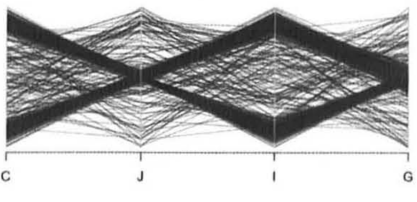
\includegraphics[width = 0.46\textwidth]{src/images/PC1}}
\qquad
\subfloat[Visual clutter inhibits cluster detection.]{\label{fig:second}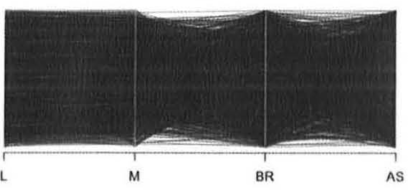
\includegraphics[width = 0.46\textwidth]{src/images/PC2}}
\caption{Parallel Coordinates without clutter and with clutter}
\end{figure}
 
 Visual clutter arises if the entire data set necessary to provide the user with an overview is displayed. Shneiderman defined the importance of overview for visualization in his mantra: \textit{"Overview first, zoom in and filter, then details on demand}  \cite{Paterno1997, Shneiderman2008, Keim2008}. Overview is a basic yet important task because it navigates the user in the data and allows further analysis. Thus, the problems of large data can be summarized as follows: 
\\*
\textit{Overlap}: 
The visualization of large data causes overlap. Depending on the drawing order the picture may look different and cause different interpretation even though the underlying data is the same. Visualization techniques need to avoid visual overlap (\ref{vis}, \ref{multi-resolution}). 
\\*
\textit{Visual Noise}: 
Even if data items are not overlapping data in large data sets might be too similar to one another. Thus, the user cannot differentiate distinct items on the screen. A solution is discussed in \ref{aggregationmarkers}.
\\*
\textit{Limited monitor resolution}:
Even if large monitors are used to visualize data in the end the available pixels on the monitor are smaller than the number of data items in a data set. This problem will be discussed in \ref{resolution}.
\\*
\textit{Limited visual perception}:
Moreover, human perception is limited in the number of patterns and pixels which will be reviewed in \ref{perception}.
\\*
\textit{Finding region of interest}:
If the data set is too large and overlap occurs the user faces the challenge of finding an interesting subset in the data. Thus, appropriate interaction techniques are necessary (\ref{search}).
\\*
\textit{Navigation}:
To find a region of interest the user might zoom in. But then another challenge occurs in navigating in the large data set. As there are too many data points the user might loose the overview and get lost in data analysis. Navigation techniques are a method to overcome this problem (\ref{navigation}).
\\*
\textit{Data Manipulation}:
If data is too large the user cannot identify whether the data is lying or not. Thus, the user may not detect data manipulation.
\\*
\textit{Information Loss}:
While reducing the number of data items to present them on the limited screen information in the data can be lost. The important question is which data characteristics to keep such that the user tasks can still be supported.
\par
To propose a solution to the problems of large-scale data visualization it is important to gain understanding of the process of visualization which is described in the Visualization Pipeline in figure\ref{fig:vispipeline}. 
\begin{figure}[H]
    \centering
        \scalebox{.5}{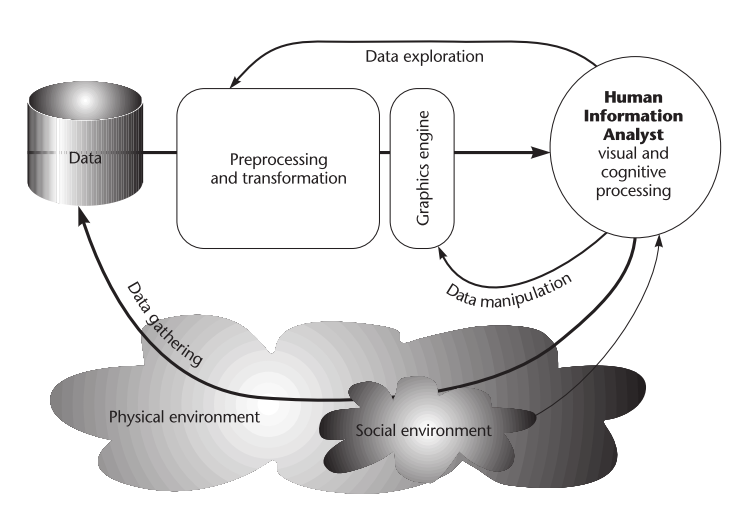
\includegraphics{src/images/VisPipeline}}
    \caption{Visualization Pipeline}
    \label{fig:vispipeline}
\end{figure}
Given the data as input visual clutter can be reduced by adapting the steps \textit{preprocessing \& transformation}, \textit{graphics engine}, \textit{visualization} and \textit{data manipulation}. Preprocessing involves data preparation such as database joins or data cleansing. The graphics engine covers rendering processes and data formats. This part will not be covered in this work as it is out of scope since the focus of this work is on visualization techniques. With visualization techniques are considered and data manipulation describes interaction techniques.  

Business visualization is used in the process of \textit{problem-solving}  \cite{Bacic2012}. Thus, the user visualizes data to gain insights into the data and to find answers to previously formulated questions.  
As the visualization pipeline shows, the process of visual analysis is influenced by three entities: the data, the user and the visualization.
The three entities can also be described as \textit{domains}: data-domain, user-domain and visualization-domain. The data-domain represents \textit{what} is visualized. The user-domain explains \textit{why} the problem is visualized and the visualization-domain characterizes \textit{how} the problem is visualized. Thus, we will now explore the three domains to answer the following questions: 

\begin{itemize}
    \item What is presented?
    \item Why is it presented?
    \item How it is presented?
\end{itemize}


% Data types for Information Visualization
\section{Data type} \label{data}

\textbf{What is presented?}\\*
Talking of large time-oriented data for business we will consider three given characteristics of data: characteristics of business data, time-dependency and its size. Business data is collected in many different areas. Table \ref{table:applications} gives an overview of the applications: 

\begin{table}[H]
	\centering
	\caption[Business Applications]{Business Applications  \cite{Brachman1996,Tegarden1999}}
	\label{businessapplications}
	\begin{tabular}{ll}
	\toprule
	Marketing & Financial Sector \\
	Fraud Detection & Manufacturing and Production \\
	Operations Planning & Market Analysis \\
	Health Care & Network Management\\
	\bottomrule
	\label{table:applications}
	\end{tabular}
\end{table}
For each application area a number of publications covering different aspects exists. The analysis of every single application would go beyond our scope so we decided to consider data with the following characteristics only: 
\begin{enumerate}
    \item Data that is structured. 
    \item Data that is abstract.
    \item Data that is multivariate.
    \item Data that is discrete.
\end{enumerate}
This selection is based on the work of Tegarden in which business data is described as abstract, multivariate and discrete  \cite{Tegarden1999}.
\textbf{Structured data}: Data can come in many different forms. Unstructured data appears in text, speech and language processing  \cite{Borgo2013}. Structured data comes in tables in which each attribute is represented by one column and each row is one data item. The attributes can be either numerical or text-based. As multivariate data is usually represented in tables  \cite{Borgo2013} we assume that business data is structured.\\*
\textbf{Abstract data}: Abstract data is defined as data without any spatial relationship in the data  \cite{Shneiderman1996}. \\*
\textbf{Multivariate data}: 
Often, multivariate is mixed-up with the term multi-dimensional. For this reason we define  multivariate data by the number of dependent attributes. If the data set holds more than two dependent attributes then we call the data \textit{multivariate}. In contrast, multi-dimensional depicts the number of independent attributes of a data set \cite{Aigner2011}.  \\*
\textbf{Discrete and time-oriented data}: A time-oriented data set contains data items which change over time. Each data item has a timestamp which is saved in one table-column. The time-dependency of the data structures the data by a given order. Every data item is mapped to a specific point in time with a smallest possible unit such as seconds. Time with a smallest unit is mapped to integer  \cite{Aigner2011} and thus we assume that time-oriented business data is discrete and has a given order.  \\*

In section \ref{vis} different techniques are compared which can display time-oriented abstract, multivariate and discrete data. 
Time-oriented data can further be differentiated into linear or cyclic, point- or interval-based and branching or multiple perspective  \cite{Aigner2011}. These factors where not considered in the selection of techniques. \\*

\textbf{Large data:} To characterize the data volume we follow a definition of Huber. He divided data into small, medium, large, huge and massive data. Large data according to  \cite{Huber1994} is defined as data sets with $10^6$ and huge data with $10^8$ data entries. We are considering large and huge amounts of data. Nowadays, companies strive to do \textit{Big Data}. Big Data in typically defined as data with  high volume, high velocity, high veracity and high variety  \cite{Wang2015}. 



% User Tasks
\section{Time-oriented User Tasks} \label{tasks}
\textbf{Why is it presented?}\\*
In the visualization analysis process the user has the role of the data analyst which is why every visualization tool should consider the user perspective. The business user is a person that is interested in verifying existing hypothesis (verification) and discover new patterns (discovery). By using the tool he expects the tool to assist him in analyzing the data, finding critical issues and perform analysis automatically  \cite{Brachman1996}. Verification and discovery in the analysis of time-oriented data can be split in seven major tasks  \cite{Esling2012}:\\*

\textbf{T1: Query by Content}
\\*
Given a known query \textit{query by content} describes the retrieval of similar items to this query. In time-oriented data query by content returns the \textit{k} most similar time series to the queried time series.
\\*
\textbf{T2: Clustering}\\*
Clustering is the process of finding expressive groups (clusters) in the data. Therefore, the data set is divided into subgroups according to some similarity measure. In the context of large time-oriented data clustering is important to compare similar time-series.
\\*
\textbf{T3: Classification}\\*
In classification the task is to find the right group the item belongs to. According to Aigner et al. temporal classification describes the preprocess of finding the correct group for given data or data set. This task is important for large data to abstract the data and make it manageable. As this task is preprocessing and not data presentation or exploration we will not check whether the tools support the user in this task. 
\\*
\textbf{T4: Segmentation}\\*
Segmentation splits a time series into \textit{k} meaningful subsequences (segments)  \cite{Batyrshin2007}. 
\\*
\textbf{T5: Prediction}\\*
In Prediction \textit{k} future events are predicted based on the past \textit{n} time series. This process is also known as \textit{forecasting}. 
\\*
\textbf{T6: Anomaly Detection} \\*
Anomaly detection points out events which behave in a different way than expected.
\\*
\textbf{T7: Pattern Discovery}\\*
Pattern discovery finds regularly appearing structures in a time series.  It covers the exploration of trends, outliers and clusters. Especially, in business this task is one of the most important tasks.

% Visualization Techniques
\section{Visualization of Time-oriented Data} \label{vis}
\textbf{How is it presented?}\\*
% introduction of methodology: selection of vizTechniques, introduction of classes
The following section discusses several visualization techniques for time-oriented data with regard to their scalability to large data sets. The choice of the technique influences the scalability which is illustrated by the following example. 
A line chart maps one dimension to the x-axis while a second dimension is mapped to the y-axis as in figure \ref{fig:linechart}. Considering, that each data items requires one screen pixel the maximum number of data items is limited by the window width. 
\begin{figure}[H]
    \centering
    \scalebox{0.2}{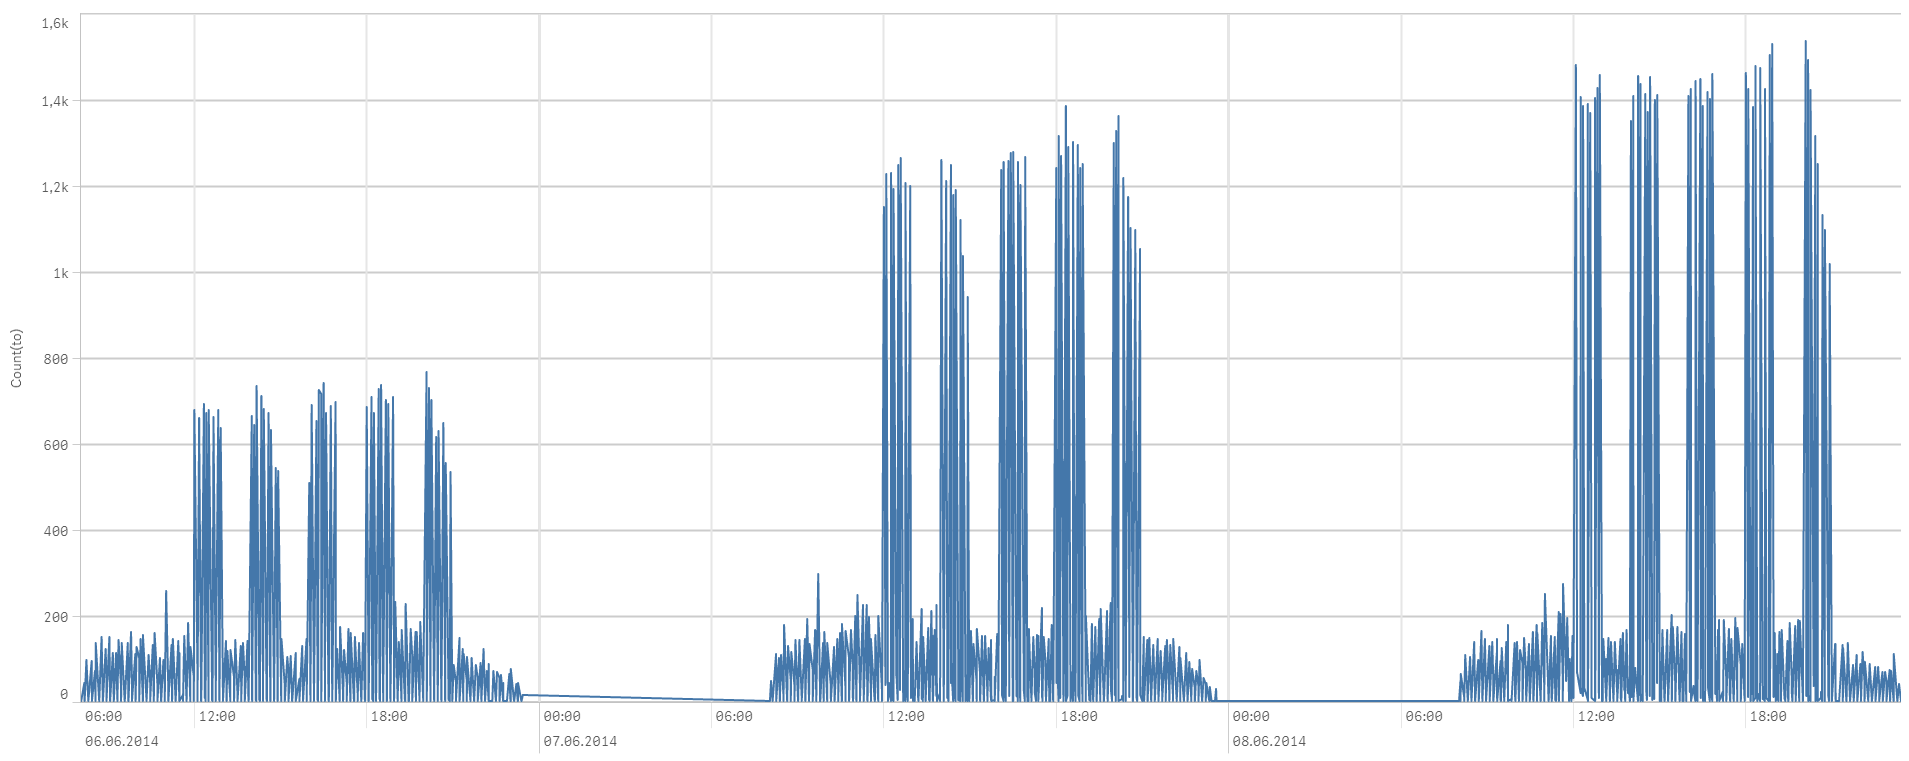
\includegraphics{src/images/linechart}}
    \caption{Linechart}
    \label{fig:linechart}
\end{figure}
 
In contrast to the line chart the scatter plot uses three attributes so the maximum number of data items in the scatter plot exceeds the maximum in the line chart which is shown in \ref{fig:scatterplot}. Hence, the technique influences the maximum number of data items that can be visualized. 
\begin{figure}[H]
    \centering
    \scalebox{0.2}{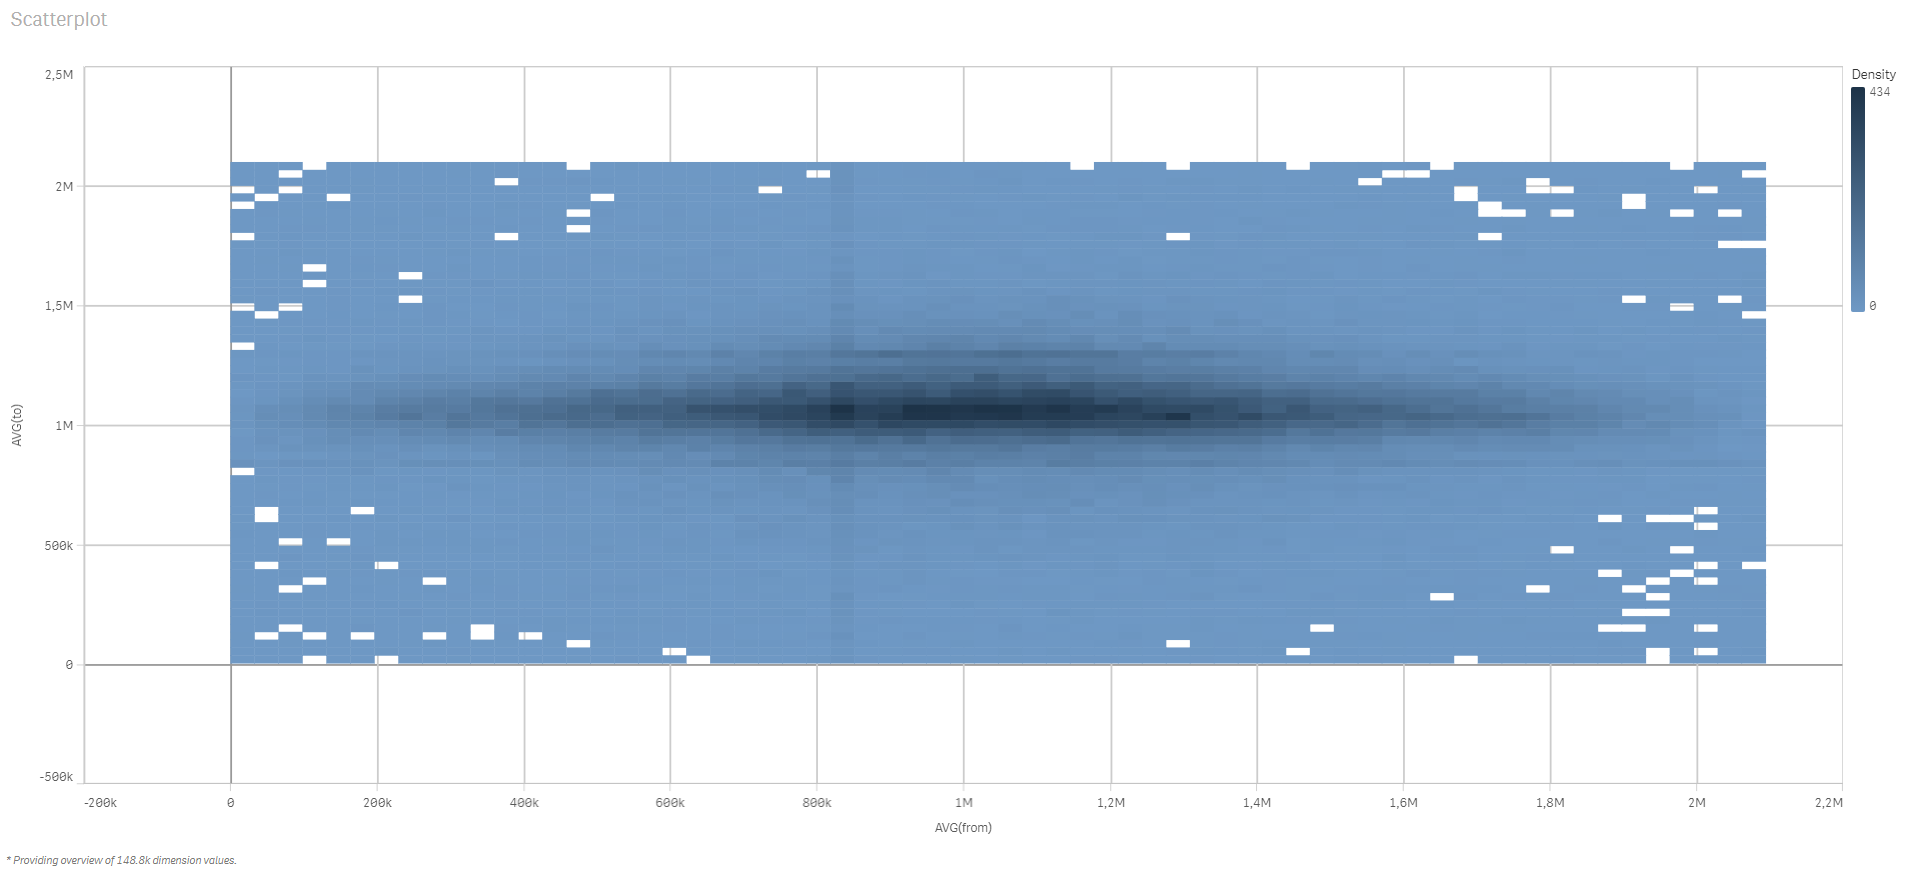
\includegraphics{src/images/SmartDataCompression}}
    \caption{Scatter plot}
    \label{fig:scatterplot}
\end{figure}
 

\textbf{Standard Visualizations of time series data:}
Usually time series data is visualized with line charts. However, line charts can only show \textit{univariate} data. Our selection of visualization techniques is based on Aigner et al.  \cite{Aigner2011} which presents current approaches to visualize time-oriented data. Hereby, we focus on 34 techniques which can be used to show abstract, multivariate and discrete data (compare section \ref{data}). 
As the work of Aigner was published in 2011 we completed the set of techniques with current approaches based on the \href{http://survey.timeviz.net/}{TimeVizBrowser} a web-based collection of time-oriented techniques. Moreover, we consider only stand-alone visualization techniques - no systems, tools or software. In literature a significant amount of publications describe new tools or systems which tackle the visualization of time-oriented data. These tools usually are specific tools which can only be applied in a limited field. As we write this work with the perspective of business users tools have to be generic and single-task systems are not appropriate.

We are aware that this discussion cannot be exhaustive as time-oriented data is a current research area and new visualization techniques are developed in rapid fashion.
Moreover, time-oriented data appears in different areas of business: E-commerce, Smart Health, E-Government, Science \& Technology, Security \& Public safety. Each sector collects different types of data and uses different applications, which makes it impossible to name every single existing visualization technique.


However, we think that this work gives a good overview of visualization techniques as we apply Keim's taxonomy  \cite{Keim1995} of visualization techniques for large data which classifies visualizations into the following classes: \textit{geometric-projective}, \textit{graph-based}, \textit{hierarchical}, \textit{icon-based} and \textit{pixel-oriented}.
\\*
\textbf{Graph-based} techniques present large graphs by using layout algorithms  \cite{Keim1996}.\\*
\textbf{Geometric projection} techniques (GP-techniques) map multi-dimensional data to the 2D screen  \cite{FerreiradeOliveira2003}.\\*
\textbf{Pixel-oriented} techniques map each data item to one pixel on the screen. Position and color are used to represent data attributes  \cite{Keim1996}.\\*
\textbf{Hierarchical} techniques divide the k-dimensional space into subspaces and shows it hierarchically. \\*
\textbf{Icon-based} techniques map each data item onto one icon. The attributes are mapped to different icon features  \cite{Keim2001}.
